\documentclass[border=10pt]{standalone}
\usepackage{tikz}\usepackage{amsmath}\usetikzlibrary{arrows.meta}
\begin{document}
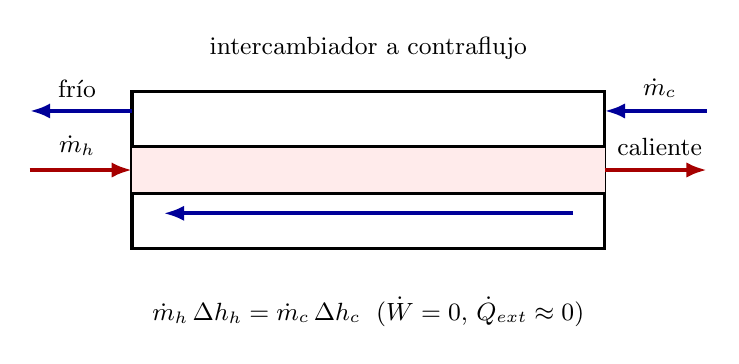
\begin{tikzpicture}[line width=1pt,>={Latex[length=2.6mm]}]
  % carcasa
  \draw[line width=1.2pt] (0,0) rectangle (6,2);
  % tubo interno (fluido caliente)
  \fill[red!8] (0,0.7) rectangle (6,1.3);
  \draw[line width=1.0pt] (0,0.7)--(6,0.7) (0,1.3)--(6,1.3);
  % caliente: izq -> der
  \draw[->,red!65!black,line width=1.5pt] (-1.3,1.0)--(0,1.0);
  \node[above] at (-0.7,1.05){\small $\dot m_h$};
  \draw[->,red!65!black,line width=1.5pt] (6,1.0)--(7.3,1.0);
  \node[above] at (6.7,1.05){\small caliente};
  % frio: der -> izq (contraflujo), por la carcasa
  \draw[->,blue!60!black,line width=1.5pt] (7.3,1.75)--(6,1.75);
  \node[above] at (6.7,1.78){\small $\dot m_c$};
  \draw[->,blue!60!black,line width=1.5pt] (0,1.75)--(-1.3,1.75);
  \node[above] at (-0.7,1.78){\small frío};
  \draw[->,blue!60!black,line width=1.4pt] (5.6,0.45)--(0.4,0.45);
  \node at (3,2.55){\small intercambiador a contraflujo};
  \node at (3,-0.8){\small $\dot m_h\,\Delta h_h = \dot m_c\,\Delta h_c$ \;($\dot W=0$, $\dot Q_{ext}\approx0$)};
\end{tikzpicture}
\end{document}
